\section{Kompression von Zeitreihen}
Übersetzt aus dem Englischen, beschreibt D. Salomon den Begriff Daten Kompression in "`Data compression: The Complete Reference"' \cite[p. 1-2]{d2004} folgendermaßen: "`\textit{Daten Kompression ist der Prozess der Konvertierung eines Eingangsdatenstroms [\ldots], hin zu einem anderen Datenstrom [\ldots] der eine kleinere Größe hat. Ein Strom ist entweder eine Datei oder ein Puffer im Speicher.}"'

Laut ihm gibt es zwei Hauptgründe warum man Daten komprimiert. Erstens ist der physische Speicher begrenzt, das heißt man möchte das Volllaufen mittels Aussortieren und Kompression so weit hinauszögern wie nur möglich, wobei das Aussortieren aufwendig sein kann als das Komprimieren. Zweitens ist der Mensch ungeduldig, das heißt man möchte viele Daten schnell übertragen können und nicht mehrere Sekunden warten bis die Daten z.B. angezeigt werden. In unserem Fall spielt der erste Grund wohl die wichtigere Rolle, da es darum geht, Zeitreihen effizient speichern zu können und sie dann zu analysieren, statt sie zu verschieben oder zu versenden.

Nachfolgend werden nun die vier verschiedene Kompressionsverfahren erläutert, die für das Experiment in \autoref{ch:experimentundergebnis} benötigt werden.

\subsection{Stückweise polynomielle Approximation}\label{subsec:ppa}
Die Idee hinter dieser Vorgehensweise ist, dass man eine Zeitreihe in gleich oder verschieden große Segmente einteilt und diese dann mit einem Polynom $n$-ten Grades approximiert. In "`Time Series Compression Survey"' \cite[Ch. 4.2.1]{gc2023} wird ein Greedy-Algorithmus beschrieben, der sukzessiv das längste Segment findet, das mit einem Polynom beschrieben werden kann, welches einen maximalen Fehler nicht überschreitet. Dem Algorithmus gibt man also die Zeitreihe, einen maximalen Grad $n$ und einen maximalen Fehler. Solange, bis die Approximation nicht mehr innerhalb des maximalen Fehlers liegt, wird die Segmentlänge schrittweise erhöht und es wird das Polynom höchsten Grades gesucht, wobei der maximale Grad $n$ nicht überschritten wird. Die beste Approximation, das heißt die längste zulässige Approximation, wird sich gemerkt und zurückgegeben.

Diese Herangehensweise ist für unser Experiment allerdings nicht geeignet. Denn einerseits müssen die Segmente gleich groß sein, da sich sonst die Koeffizienten auf verschiedene Definitionsbereiche beziehen und somit nicht vergleichbar sind, andererseits können wir den Grad der Polynome nicht beliebig machen, da sonst die Koeffizienten nicht miteinander vergleichbar sind. Dass die Koeffizienten von Polynomen verschiedenen Grades nicht vergleichbar sind, ist an dem simplen Beispiel von $P_1(x)=x^2+x$ und $P_2(x)=x^3+x^2+x$ zu sehen. In \autoref{fig:PolynomeVerschiedeneGrade} sieht man, dass obwohl die Koeffizienten von $x$ und $x^2$ identisch sind, macht das zusätzliche $x^3$ bei $P_2$ einen großen Unterschied. Für unser Experiment müssen wir also eine feste Segmentlänge und einen festen Grad für das Polynom festlegen. Außerdem legen wir keinen maximalen Fehler fest, sondern suchen das Polynom mit dem least squares fit \cite[Def. least squares fitting]{end}. Das bedeutet, dass wir das Polynom $P(x)$ suchen, mit der kleinsten Quadratsumme $\sum_i (P(x_i)-y_i)^2$, wobei die Punkte $(x_i,y_i)$ den Datenpunkten aus der Zeitreihe entsprechen.
\begin{figure}[bth] 
  \centering
  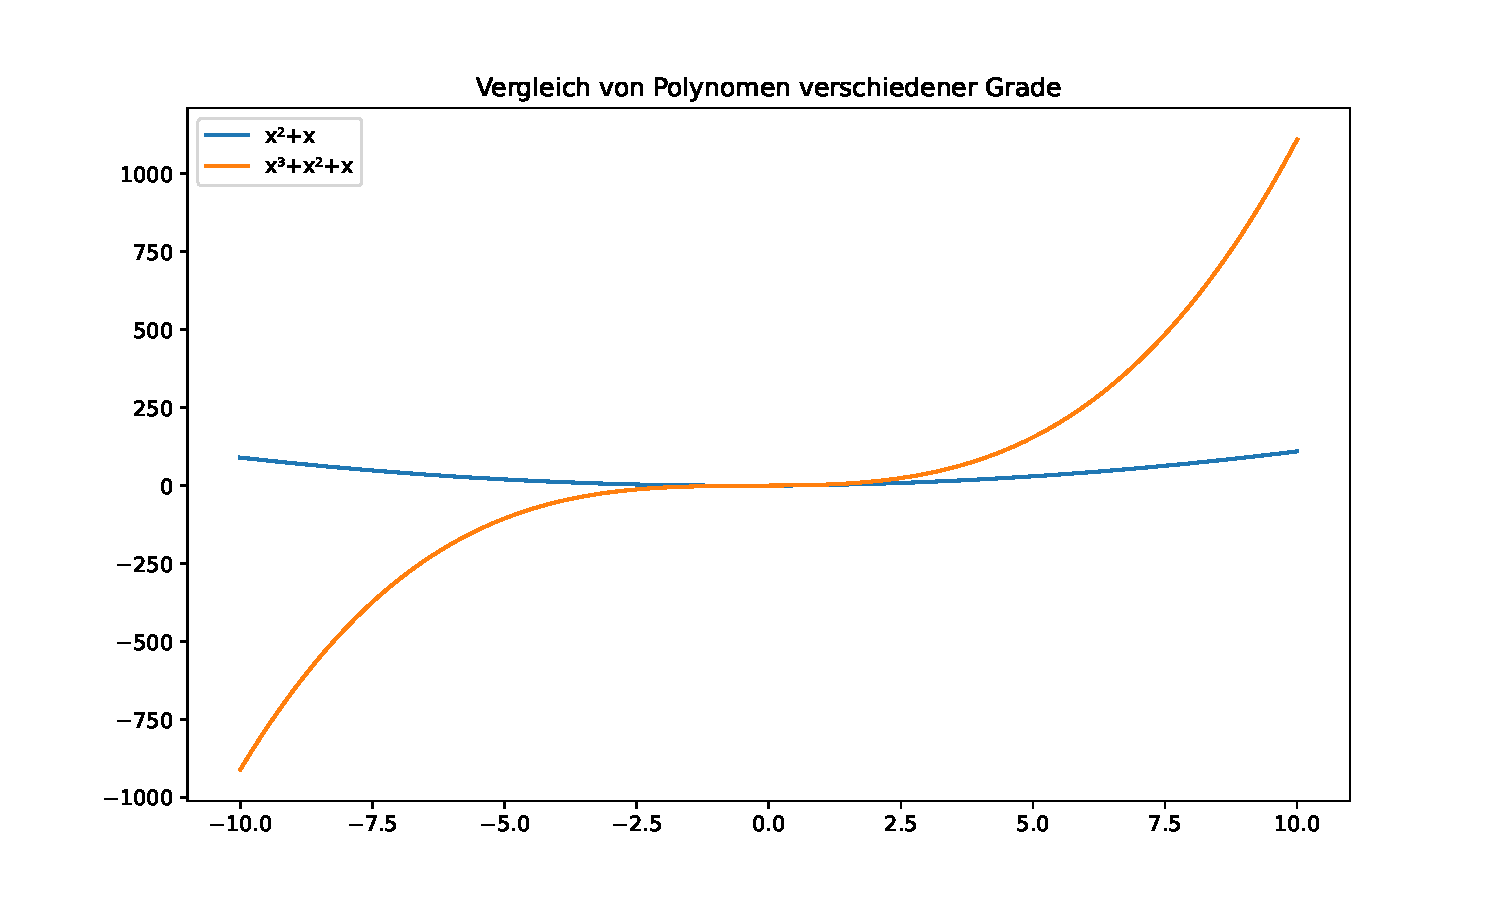
\includegraphics[width=0.7\textwidth]{Graphics/ComparissonDifferentPolDegrees.pdf}
  \caption{Vergleich von Polynomen verschiedener Grade}
  \label{fig:PolynomeVerschiedeneGrade}
\end{figure}

\subsection{Stückweise lineare Approximation}
Die stückweise lineare Approximation stellt einen Spezialfall der stückweisen polynomiellen Approximation dar, bei dem ausschließlich Polynome ersten Grades (also lineare Funktionen) zur Approximation der Segmente verwendet werden.
Durch die Beschränkung auf Grad 1 ergibt sich eine einfachere Funktionsform sowie geringerer Rechenaufwand, jedoch unter Umständen auch eine schlechtere Approximation komplexer Verläufe im Vergleich zu höhergradigen polynomiellen Approximationen.

\subsection{Diskrete Fourier-Transformation}
Die \ac{DFT} ist ein mathematisches Verfahren zur Zerlegung einer endlichen, diskreten Zeitreihe in ihre Frequenzteile. Das heißt für eine gegebene Zeitreihe $[(t_0,x_0),(t_1,x_1),\ldots,(t_{n-1},x_{n-1})]$, gibt \acs{DFT} eine neue Liste, mit den Frequenzen von 1 bis $n$, zurück. Für diese Transformation ist folgende Formel definiert:
\[y_k=\sum_{\ell=0}^{n-1}x_\ell\,e^{-i\,\tfrac{2\pi k}{n}\,\ell},\]
wobei $[y_0,y_1,\ldots,y_{n-1}]$ die neue Liste ist und $i$ die imaginäre Einheit.

Was dieses Verfahren tut, lässt sich gut an einem Beispiel zeigen. In \autoref{fig:dftKomplettBeispiel} sieht man in Grün ein Signal, das aus drei sich überlagernden Frequenzen erstellt wurde. Die blauen Punkte sind zwölf Messpunkte einer Zeitreihe, die dieses Signal abgetastet hat, und die gelben Kreuze sind das Ergebnis der \acs{DFT}. 
\begin{figure}[bth] 
  \centering
  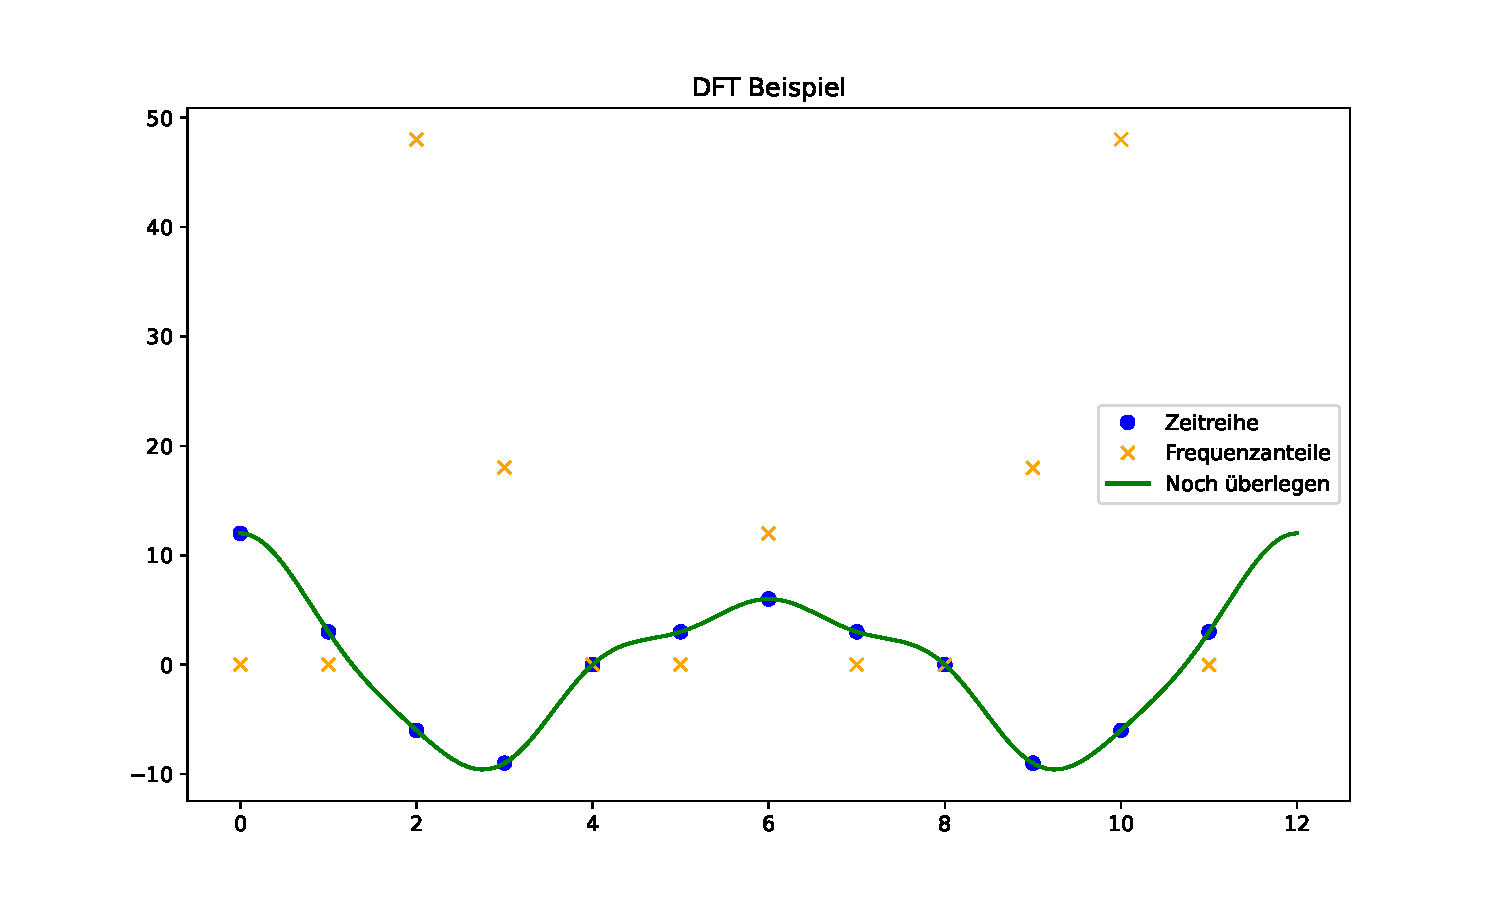
\includegraphics[width=0.7\textwidth]{Graphics/DFTExample1.pdf}
  \caption{Beispiel einer diskreten Fourier"=Transformation}
  \label{fig:dftKomplettBeispiel}
\end{figure}

\begin{figure}[bth]
  \subfloat[Erstes ...]{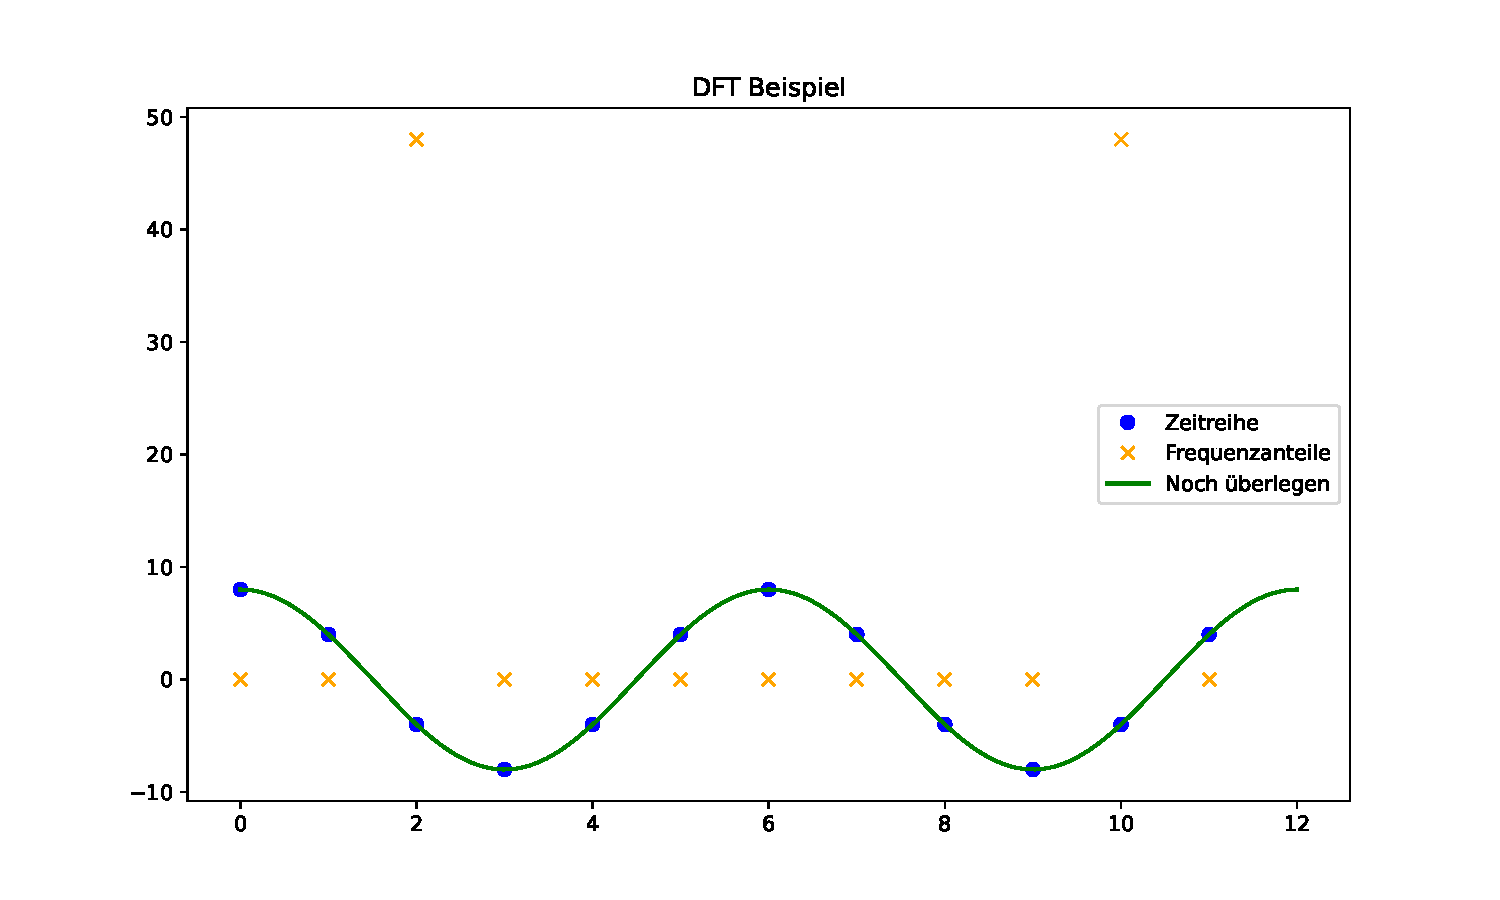
\includegraphics[width=0.49\textwidth]{Graphics/DFTExample4.pdf}\label{subfig:dft2}}\hfill
  \subfloat[... und zweites Bild]{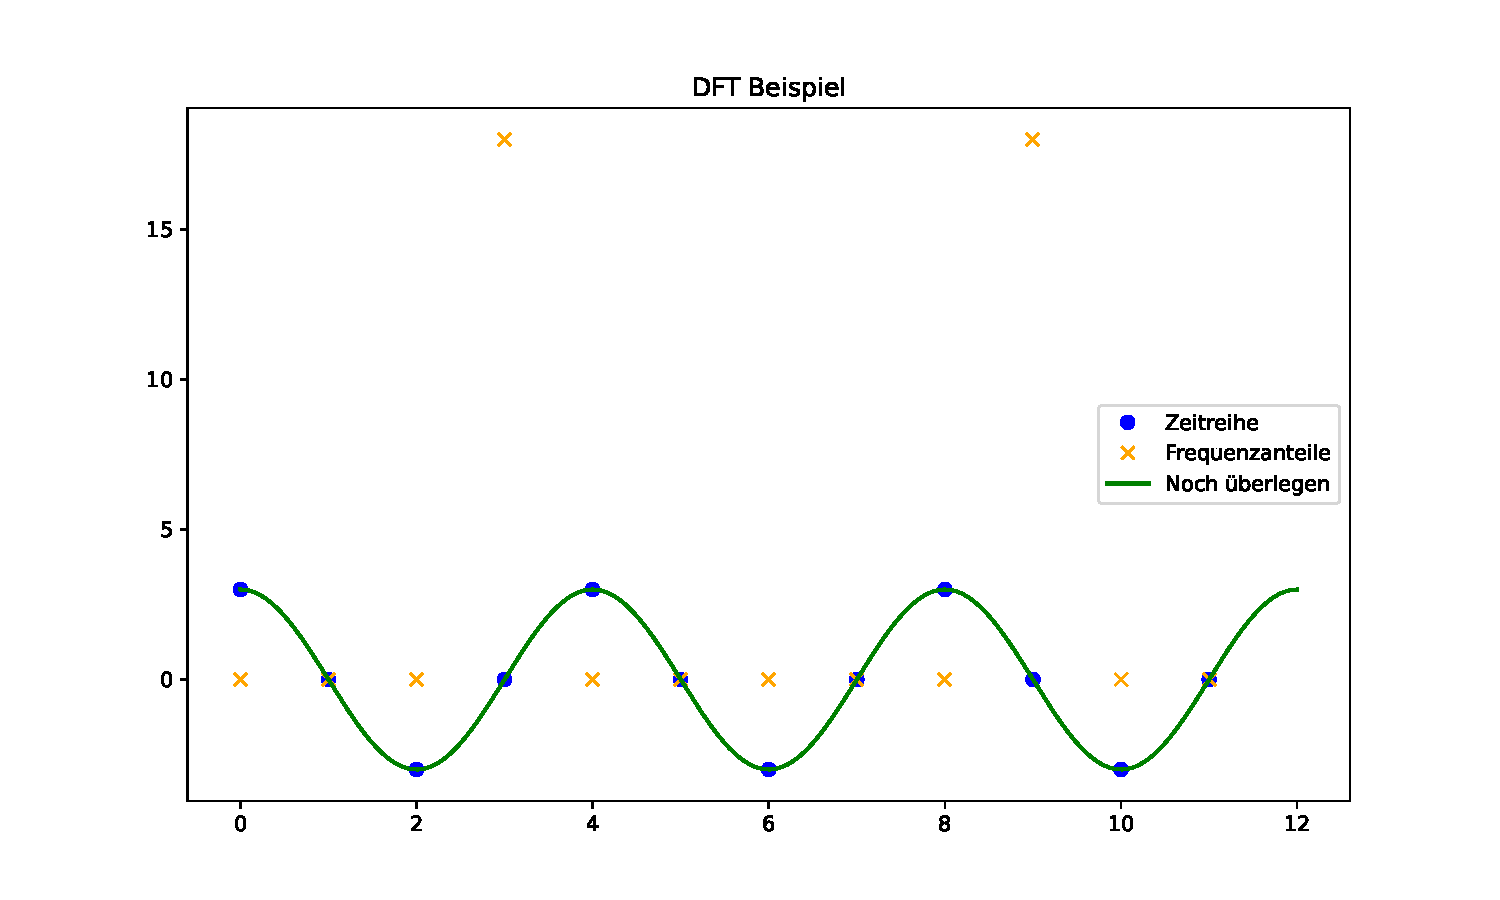
\includegraphics[width=0.49\textwidth]{Graphics/DFTExample3.pdf}\label{subfig:df3}}\hfill
  \centering\subfloat[... und drittes Bild]{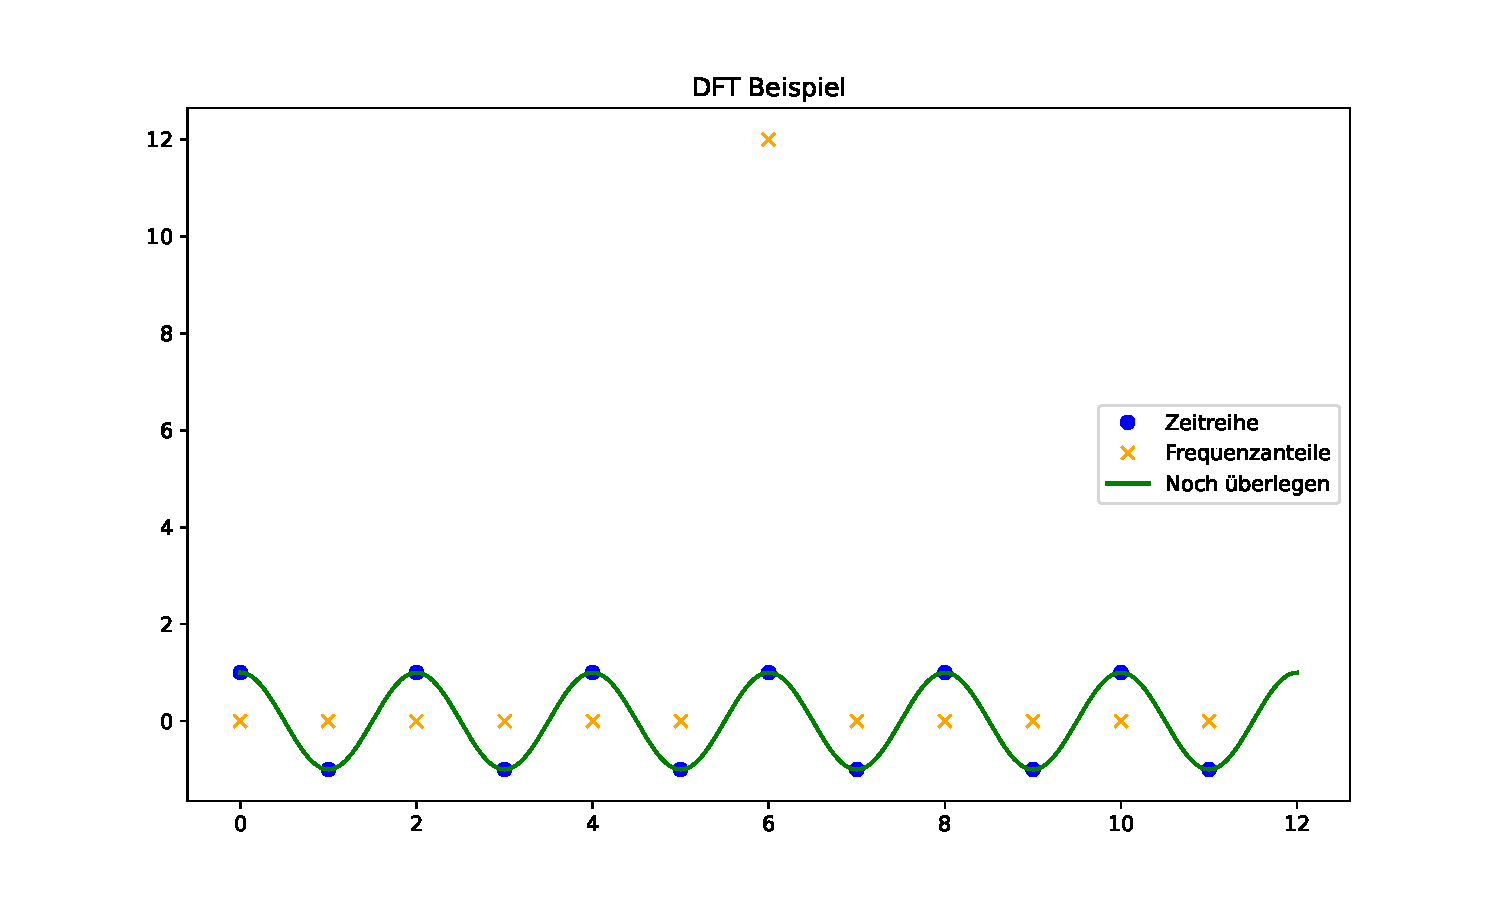
\includegraphics[width=0.49\textwidth]{Graphics/DFTExample2.pdf}\label{subfig:dft4}}
  \caption{Mehrere Abbildungen nebeneinander}
  \label{fig:dftEinzelneFrequenzen}
\end{figure}

Zum besseren Verständnis der am Anfang genannten Formel wird in diesem Abschnitt nun näher auf die Mathematik dahinter eingegangen. In der Formel handelt es sich wegen der imaginären Einheit $i$ um komplexe Zahlen. Diese bestehen aus einem Real Teil $a$ und einem Imaginär Teil $b$, also in der Form $a + ib$. Sie können allerdings auch als Punkt in einer zweidimensionalen Ebene interpretiert werden, dann liegt der Real Teil typischerweise auf der x-Achse und der Imaginär Teil auf der y-Achse. Außerdem gibt es die Exponentialform $a+ib=re^{i\varphi}$, wobei $r$ der Abstand vom Ursprung zum Punkt $(a,b)$ ist und $\varphi$ der Winkel den diese Strecke mit der x-Achse einschließt. $r$ wird auch Betrag genannt und wird folgendermaßen berechnet: $r=\sqrt{a^2+b^2}$. 